\documentclass[tikz,border=4pt]{standalone}
\usetikzlibrary{arrows.meta, positioning, calc}
\definecolor{patch}{HTML}{1F77B4}
\definecolor{sham}{HTML}{FF7F0E}
\begin{document}
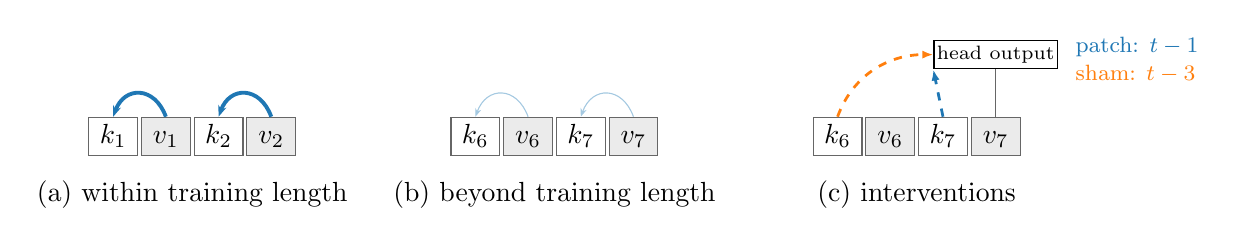
\begin{tikzpicture}[
    tok/.style={draw=black!60, line width=0.4pt, minimum width=0.62cm, minimum height=0.48cm, inner sep=0pt,
                text height=1.6ex, text depth=0.4ex},
    val/.style={tok, fill=black!8},
    attend/.style={-{Stealth[length=4pt]}, line width=1.4pt, patch},
    faint/.style={-{Stealth[length=3pt]}, line width=0.4pt, patch!40},
    write/.style={-{Latex[length=4pt]}, line width=1pt, dashed},
    slot/.style={draw=black, line width=0.5pt, minimum width=1.2cm, minimum height=0.36cm, inner sep=1pt,
                 font=\scriptsize},
    subcap/.style={anchor=north},
  ]
  \begin{scope}
    \node[tok] (a1) at (0,0) {$k_1$};
    \node[val, right=1pt of a1] (a2) {$v_1$};
    \node[tok, right=1pt of a2] (a3) {$k_2$};
    \node[val, right=1pt of a3] (a4) {$v_2$};
    \draw[attend] (a4.north) to[out=110, in=70, looseness=1.6] (a3.north);
    \draw[attend] (a2.north) to[out=110, in=70, looseness=1.6] (a1.north);
    \node[subcap] at ($(a2.south)!0.5!(a3.south)+(0,-0.2)$) {(a) within training length};
  \end{scope}

  \begin{scope}[xshift=4.6cm]
    \node[tok] (b1) at (0,0) {$k_6$};
    \node[val, right=1pt of b1] (b2) {$v_6$};
    \node[tok, right=1pt of b2] (b3) {$k_7$};
    \node[val, right=1pt of b3] (b4) {$v_7$};
    \draw[faint] (b4.north) to[out=110, in=70, looseness=1.6] (b3.north);
    \draw[faint] (b2.north) to[out=110, in=70, looseness=1.6] (b1.north);
    \node[subcap] at ($(b2.south)!0.5!(b3.south)+(0,-0.2)$) {(b) beyond training length};
  \end{scope}

  \begin{scope}[xshift=9.2cm]
    \node[tok] (c1) at (0,0) {$k_6$};
    \node[val, right=1pt of c1] (c2) {$v_6$};
    \node[tok, right=1pt of c2] (c3) {$k_7$};
    \node[val, right=1pt of c3] (c4) {$v_7$};
    \node[slot, above=0.6cm of c4] (o) {head output};
    \draw[black!60, line width=0.4pt] (c4.north) -- (o.south);
    \draw[write, patch] (c3.north) -- (o.south west);
    \draw[write, sham] (c1.north) to[out=70, in=180] (o.west);
    \node[font=\footnotesize, text=patch, anchor=west] at ($(o.east)+(0.1,0.1)$) {patch: $t-1$};
    \node[font=\footnotesize, text=sham, anchor=west] at ($(o.east)+(0.1,-0.25)$) {sham: $t-3$};
    \node[subcap] at ($(c2.south)!0.5!(c3.south)+(0,-0.2)$) {(c) interventions};
  \end{scope}
\end{tikzpicture}
\end{document}
